\section{Обзор существующих решений}
\label{sec:Chapter2} \index{Chapter2}

\subsection{Формат сигнатур}

Прежде чем говорить непосредственно о методах автоматической генерации сигнатур, стоит сначала понять какие бывают сигнатуры и в каком формате они будут представлены.

Существует несколько представлений сигнатур. Некоторые из этих видов использовались для представлений сигнатур червей.
Однако для обычного трафика можно выделить два основных представления:

\begin{enumerate}
    \item сигнатуры, представленные регулярными выражениями
    \item сигнатуры, представленные строками
\end{enumerate}

Использование регулярных выражений для описания сигнатур приложений становится очень распространнённым в классификации потоков.
Однако процесс сопоставления регулярных выражений требует огромной вычислительной мощности, которая не масштабируется для идентификации сетевого трафика в режиме реального времени.
Способ построения регулярного выражения оказывает непосредственное влияние на классификацию потоков и на общую производительность сопоставления.
Несмотря на это, некоторые системы DPI используют регулярные выражения для представления сигнатур приложений. Система обнаружения/предотвращения вторжений Snort (IDS/IPS)
имеет более 1000 подписей приложений и предлагает пользователю возможность вставлять новые регулярные выражения по требованию.

Представление сигнатур в виде строк это компромисс между мощностью выражения и эффективностью сопоставления.
Также такой подход позволяет преобразовывать сигнатуры, представленные строками, в регулярные выражения.

Будем дальше рассматривать сигнатуры в виде строк, преобразование в регулярные выражения останется за рамками данной работы.

\subsection{Структура сигнатур}

Большинство форматов сигнатур в предыдущих работах представляют собой простые подстроки, которые часто появляются в полезной нагрузке.
Следовательно, всё ещё существует вероятность того, что извлеченные сигнатуры полезной нагрузки могут быть не специфичными для конкретного приложения,
некоторые могут принадлежать и другому приложению. Это называется избыточностью сигнатур.

Выделим три типа сигнатур:

\begin{enumerate}
    \item сигнатура содержимого (полезной нагрузки),
    \item сигнатура пакета,
    \item сигнатура потока.
\end{enumerate}

\begin{figure}[H]
    \begin{center}
        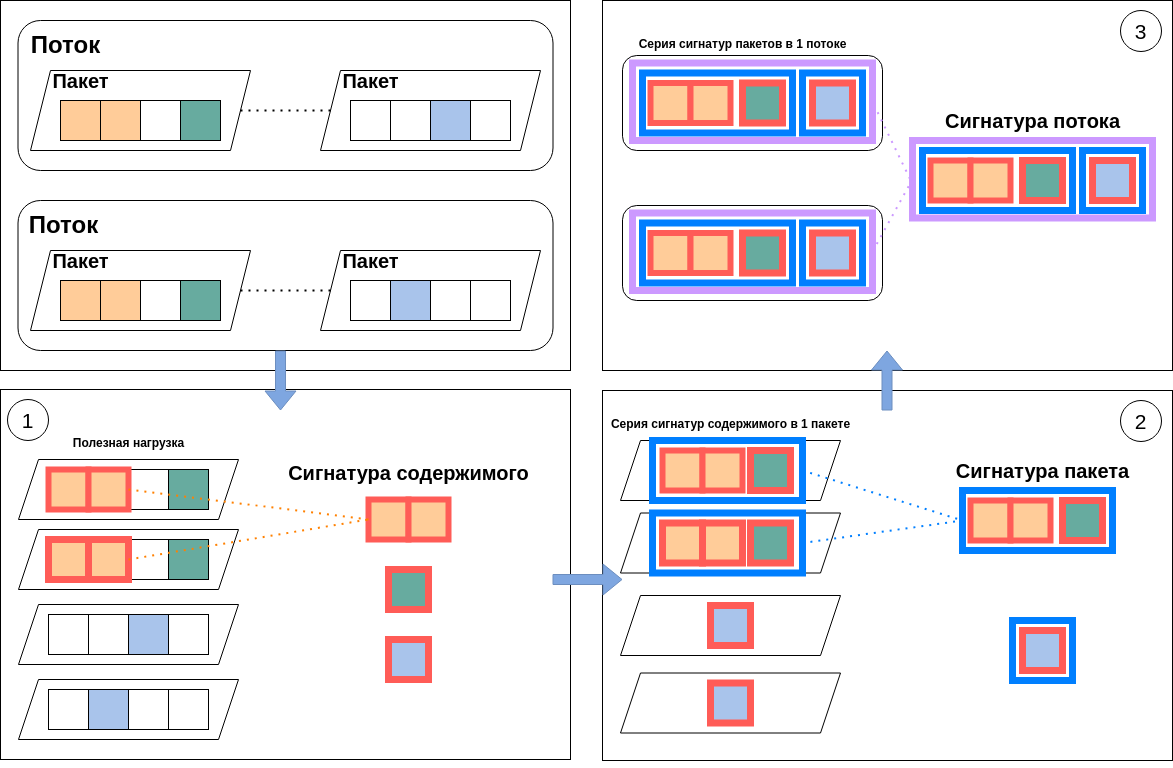
\includegraphics[width =\textwidth]{signature_structure.png}
        \caption{Процесс извлечения предлагаемой структуры сигнатур полезной нагрузки}
    \end{center}
\end{figure}

Сигнатура содержимого определяется как различимая и уникальная подстрока полезной нагрузки, состоящая из непрерывных символов или шестнадцатеричных значений.
На самом деле уникальность с помощью одной подстроки тяжело обеспечить, например, такие строки "GET" или "HTTP", которые часто встречаются в HTTP,
не могут служить конечными сигнатурами, так как они не различают приложения.

Сигнатура пакета состоит из серии сигнатур содержимого, которые появляются в одном пакете.
Так как классификация может выполняться без накопления пакетов, т.е. без сбора потока, то анализируется всегда хотя бы один пакет.
Это значит, что для классификации не имеет смысла использовать отдельно сигнатуру содержимого.

Сигнатура потока состоит из серии сигнатур пакетов, которые появляются в одном потоке, где под потоком понимается набор пакетов, имеющий одни и те же
IP-адресс источника, IP-адресс назначения, порт источника, порт назначения и используемый протокол транспортного уровня.
Сигнатура потока гораздо более специфична для конкретного приложения, чем сигнатура пакета, и значительно повышает точность.

\subsection{Метрики оценки качества сигнатур}

Для оценки качества получаемых сигнатур рассмотрим матрицу ошибок: 4 стандартные категории, к котором можно отнести результат работы классификатора на полученной сигнатуре.
В нашем случае рассматриваемый класс это целевой протокол или приложение.
Под классификацией трафика будем понимать классификацию конкретного пакета или потока в зависимости от того, какой уровень сигнатур используется.

\begin{table}[H]
\centering
\resizebox{\columnwidth}{!}{
    \begin{tabular}{|c|c|c|}
    \hline
                                                      & Принадлежит классу (P) & Не принадлежит классу (N) \\ \hline
    Предсказана принадлежность к классу (T)           & TP                     & TN                        \\ \hline
    Предсказано отсутствие принадлежности к классу(F) & FP                     & FN                        \\ \hline
    \end{tabular}
}
\end{table}

\begin{itemize}
    \item истинно положительный (TP): указывает, что трафик правильно классифицирован, как относящийся к определенному классу.
    \item истинно отрицательный (TN): указывает, что трафик правильно классифицирован, как не относящийся к определенному классу.
    \item ложно положительный (FP): указывает, что трафик неправильно классифицирован, как относящийся к определенному классу.
    \item ложный отрицательный (FN): указывает, что трафик неправильно классифицирован, как не относящийся к определенному классу.
\end{itemize}

Наиболее часто используемые показатели для классификации трафика определяются следующим образом:

\begin{itemize}
    \item Accuracy (достоверность) $ = \frac{TP + TN}{TP + TN + FP + FN}$ - доля правильных классификаций.
    \item Recall (полнота) $ = \frac{TP}{TP + FN}$ - отношение верно классифицированного трафика определенному классу к общему числу трафика этого класса,
    т.е. описывает способность сигнатуры обнаружить данный целевой протокол или приложение.
    \item Precision (точность) $ = \frac{TP}{TP + FP}$ - доля верно классифицированного трафика среди всего трафика, который классификатор отнёс к этому классу.
    \item F-мера = $ 2 \frac{recall \cdot precision}{recall + precision}$ - гармоническое среднее между точностью и полнотой.
    Метрика accuracy может терять свой смысл в задачах с сильно неравными классами.
    Напротив же recall и precision не зависят от соотношения классов и поэтому применимы в случае несбалансированных классов,
    что является правдой для сетевого трафика. Часто на практике возникает задача найти оптимальный баланс между precision
    и recall. Для этих целей подходит F-мера, которая достигает максимума при recall
    и precision равным 1, и стремится к минимуму, если хотя бы один из параметров стремится к нулю.
\end{itemize}

Для сигнатур полезно ещё ввести такое понятие как:

\begin{itemize}
    \item Redundancy (избыточность) опредялется как:
    $$ \text{Redundancy} = \cfrac{\text{Объём трафика идентифицированный двумя и более сигнатурами}}{\text{Объём трафика идентифицированый набором сигнатур}}$$
    Redundancy имеет значение от 0 до 1, где 0 - наилучшее значение, которое указывает на то, что все сигнатуры набора классифицируют исключительно только свою часть трафика,
    т.е. являются уникальными и незаменяемыми. Если redundancy близка к 1, то в наборе присутствует ненужные сигнатуры, которые идентифицируют перекрывающийся трафик.
    По мере увеличения количества сигнатур увеличиваются и накладные расходы системы, поэтому данное значение должно оставаться низким.
\end{itemize}

\subsection{Обзор существующих методов автоматической генерации сигнатур}

\newpage
